\documentclass{article}

\usepackage{amsmath}
\usepackage{graphicx}

\begin{document}

\title{Bayesian Particle Filter Tracking with CUDA}
\author{Geoffrey Ulman\\
        CSI702}
\date{April 2010}
\maketitle

\tableofcontents

\section{Background}
A simple geographic tracking problem traditionally consists of estimating the state of a target using errored observations of some function of the target state. The problem explored here assumes a four-dimensional state space with two cartesian position dimensions and two veocity dimensions. To simplify the problem, the possibility of false alarms (observations which do not corrispond to an actual target) is ignorred. Further, all observations are assumed to corrispond to a single target of interest (associating observations with the correct target track is an additional complicating concern in multi-target tracking problems).

\subsection{Prior Distribution}
Employing bayesian tracking to estimate the true state \(x \in S\) of a target in state space \(S\) requires a prior distribution \(p(x)\). This probability density function describes the probability that the target's true state is \(x\) prior to receving any observations on the target. This prior distribution is generally based on engineering knowledge of the targets and of the sensors used to generate observations. The simple priors used in this tracking problem assume the sensor has a maximum detection range and thus that targets will not be detected until they are inside that range. The velocity dimension of the target state is also restricted by the known maximum speed of the target being tracked. Together, these form a simple uniform bounded prior distribution on the two position and two velocity state space dimensions. Figure \ref{prior} displays the x and y position components of a random sample of particles drawn from the prior described above with a 20000 meter maximum detection range. Because all particles are initially weighted equally, any particle has an equal likelihood of being the true state of the target.

\begin{figure}
\centering
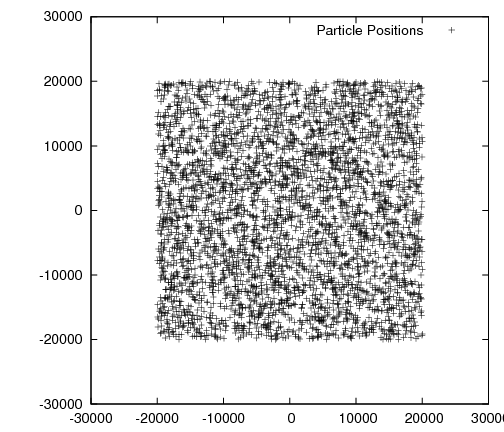
\includegraphics[width=0.7\textwidth]{data/particles_prior.png}
\caption{Prior Particle Position Distribution}
\label{prior}
\end{figure}

\subsection{Likelihood Functions}


\subsection{Motion Model}


 employs Bayes' Theorem to combine errored observations on functions of a state space \(S\) into a posterior distribution p

\section{Design}
Text...
\subsection{Parallel Reduction}
The thrust library provides prewritten parallel algorithms for common CUDA tasks, including reducing an array of values to a single value through repeated application of a binary reduction function.\cite{thrust}

My parallel array summation implementation is based on the NVIDIA white paper on the subject included in the CUDA SDK.\cite{oprc} Understanding the overall summation algorithm requires first understanding the basic shared memory summation algorithm for a single block. A simple fan-in reduction is used. At the first iteration, the first \(\frac{blockDim.x}{2}\) threads in the block add their shared memory value to the shared memory value of their counterpart in the second half of the block. The second iteration continues using \(\frac{blockDim.x}{4}\) threads, and so on. Each iteration is synchronized using \verb!__syncthreads()!. Although the values to be summed are passed to the kernel using global memory, each block immediately copies its values to shared memory and performs the rest of the reduction there. Because shared memory is hundreds of times faster than global memory\cite{tutorial1} this strategy is necessary for adequate performance.

However, the loop construct that controls this iteration is expensive, as are the \verb!__syncthreads()! calls. Fortunately, we can take advantage of the specifics of the NVIDA hardware to get substatial additional savings once the number of values in shared memory to sum drops below 32. CUDA threads are grouped into \emph{warps} of 32 threads which execute commands simultaniously as a single operation on the GPU (and thus require no synchronization). Therefore, by stopping the reduction iteration and unrolling the final iterations, we can avoid synchronization for the iterations where all the summations are occuring simultaniously automatically.

As each block completes its parallel summation, it writes its sum to an array in global memory. Thus, after the first iteration, the global memory result array will contain one value for each block. To sum these values, the kernel is called iteratively until fewer value remain than the number of threads in a single block. At this point, the kernel is called one last time with a single block which writes the final overall sum to global memory.

\begin{figure}
\centering
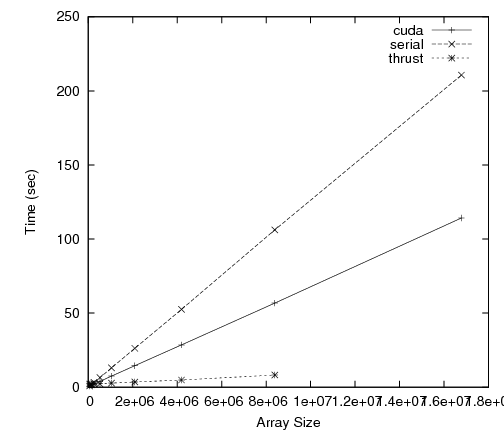
\includegraphics[width=0.7\textwidth]{data/summation_plot.png}
\caption{Array Summation Algorithm Performance}
\label{summation_plot}
\end{figure}

However, as Figure \ref{summation_plot} indicates, writing complex parallel algorithms in cuda efficiently is very difficult. Performance for the serial implementation, custom cuda implementation, and thrust implementation all scale linearly with array size, which makes sense given that the array summation problem has \(O(n)\) time complexity. What is striking is the difference in performance between the custom cuda implementation and the thrust implementation. For the largest arrays tested, the custom cuda implementation was only about twice as fast as the serial implementation whereas the thrust implementation was 12.9 times faster. These results highlight cuda's sensitivity to subtle factors like uncoalesced memory access, shared memory bank conflicts (threads from multiple warps accessing the same sections of shared memory), expensive gpu operations, and other performance gotchas which can have significant impact on performance\cite{bestprac}.

\subsection{Random Number Generation}
Particle filter tracking is a stochastic process: as particles are time updated, they maneuver randomly according to their motion model; as particles are resampled, their replacements are randomly perturbed copies of existing particles. Thus, performing particle filter tracking using CUDA required generating random numbers efficiently on the GPU. The thrust library provides random number generation capabilities, and the CUDA SDK provides a parallel MersenneTwister example. My random number generator implementation is a simpler linear congruential generator which relies on independent seeds stored for each particle.

\begin{equation}\label{lcgeq1}
X_{n+1}=(aX_{n}+c \mod m)
\end{equation}

With properly chosen \(a\), \(c\) and \(m\) values linear congruential generator can provide sufficiently random values for particle filtering\cite{lcg}. The values I used are those used by the java.util.Random class. This approach is attractive because it is theoretically very fast and requires very little state, allowing each particle to generate its own independent stream of random values. Unfortunately, the recurrence relation in equation \ref{lcgeq1} relies on the modulus operator, which is extremely slow on NVIDA hardware.\cite{oprc}

\section{Performance}
Text...

\section{Conclusion}
Text...

\begin{thebibliography}{9}

\bibitem{cpl}
  Brian W. Kernighan and Dennis M. Ritchie,
  \emph{The C Programming Language},
  Prentice Hall PTR, New Jersey,
  2009.

\bibitem{bmtt}
  Stone, Barlow, and Corwin,
  \emph{Bayesian Multiple Target Tracking},
  Artech House, Boston,
  1999.

\bibitem{oprc}
   Harris, Mark,
   \emph{Optimizing Parallel Reduction in CUDA},
   NVIDIA Developer Technology \\
   http://developer.download.nvidia.com/compute/cuda/sdk/website/samples.html

\bibitem{tutorial1}
   Volume I: Introduction to CUDA Programming \\
   http://www.nvidia.com/docs/IO/47904/VolumeI.pdf

\bibitem{bestprac}
   CUDA Best Practices Guide -- CUDA 2.2\\
   http://developer.download.nvidia.com/compute/cuda/2\_3/\\
   toolkit/docs/NVIDIA\_CUDA\_BestPracticesGuide\_2.3.pdf

\bibitem{thrust}
   Thrust C++ Template Library for CUDA \\
   http://code.google.com/p/thrust/

\bibitem{lcg}
   Linear Congruential Generator \\
   http://en.wikipedia.org/wiki/Linear\_congruential\_generator

\end{thebibliography}

\end{document}
